\subsection{System and Failure Model}\label{subsec:failure_model}
Each session has an Owner serializing selected transitions, workers
executing frozen calls, and an actual Consumer applying selected facts
and complete provisional hypotheses. Durable storage records the
selected prefix. A Supervisor monitors the processes and preserves the
accepted-input ledger.

We assume one trusted Owner per session, protected selection, immutable
audio and model configuration, unambiguous encoding, collision-resistant
digests, and storage honoring successful synchronization. Used calls must
faithfully consume their frozen inputs. Host receipts bind API objects,
not GPU arithmetic; independent Private and Authority floating-point
executions need not agree.

The interface checks identity, completeness, derived state, and ancestry.
Native resilience supports worker or Owner-group fail-stop on an intact
filesystem; Supervisor, accepted-input ledger, actual Consumer, power
observer, and synchronized storage survive. Their original input clocks
continue through restart. Supervisor/Consumer failure, host power loss,
compromised Owner or Authority, Byzantine code, persistent corruption,
and lost storage are excluded. Controlled wrong-input injections in
Section~\ref{sec:eval} intentionally violate normal Private input fidelity;
we use them to study containment and executor release, not as examples
covered by the lawful-continuation proposition.

\subsection{Feedback creates an execution dependency}
An immutable audio stream supplies a protected selection path producing
\emph{Canonical} facts and a faster \emph{Private} path computing and
displaying provisional hypotheses. Selection can change the next call's
input: StreamCorrect feeds its chosen correction into subsequent
ASR~\cite{vu2026streamcorrect}. We coordinate this dependency as the paths
advance asynchronously.

For a fixed session and execution contract, write an installed fact as
\begin{equation}
 C=(v,F,Z_C,P_C,T_C).
 \label{eq:canonical}
\end{equation}
Here $v$ is the version, $F$ the certified processing frontier, $Z_C$ the
complete selected output, $P_C$ the feedback state, and $T_C$ its bound
text. The contract fixes the model, adapter, decoding, audio identity,
and transformations to $P$ and $T$. Consumer coverage follows the adapter's
publication policy; advancing $F$ need not add characters. Certification
means acceptance by protected selection and installation, separately
from human-transcription accuracy.

The adapter declares a conservative representation of \emph{all mutable
cross-call state that can affect later model inputs, selection, or feedback}.
Telemetry and resources are separate. Qwen passes prompt tokens without
cross-call numerical KV caches. The native adapter additionally carries
audio buffers, token groups, context, alignment position, and decoder
configuration. Comparisons require the same contract: text equality
cannot replace an omitted cursor or numerical cache. The representation
may conservatively include fields unnecessary to a particular call.

\begin{figure*}[t]
\centering
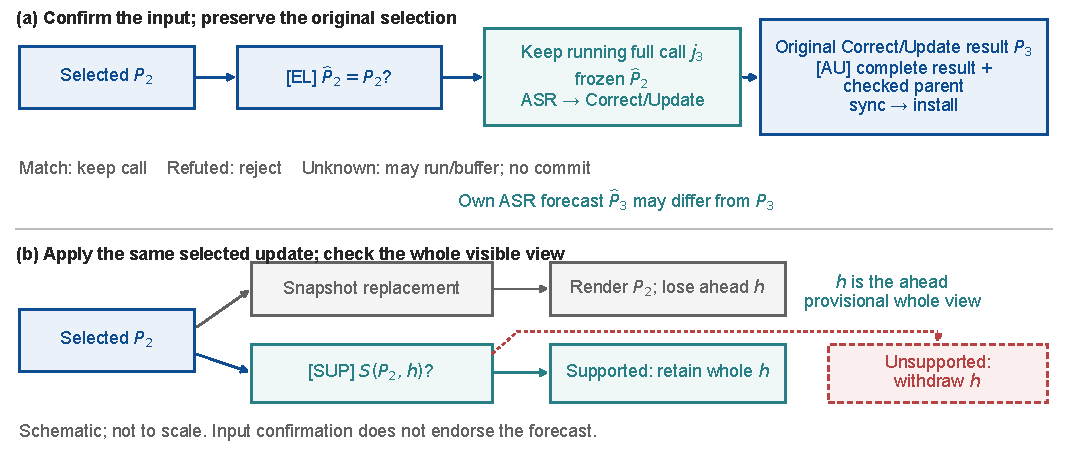
\includegraphics[width=\textwidth]{figures/coordination_protocol.pdf}
\caption{One trusted revision requires separate decisions about work and
its use. [EL] confirms the complete frozen input of $j_3$ against actual
selected $P_2$. [AU] retains original Correct/Update before durable
selection; the call's own prediction can differ from its result.
[SUP] independently retains the whole supported view when $P_2$ installs.
Unknown input remains unresolved while owned calls may run or buffer;
it grants no commit authority. Arrows show decisions and their outcomes;
the dashed red branch marks failed support. This is a causal schematic
without a measured time scale.}
\label{fig:protocol}
\end{figure*}

\subsection{Calls, views and outstanding input}
A complete provisional node $n$ records a frozen call
\begin{equation}
 q_n=(a_n,P_n^-,b_n,\chi_n),\quad
 n=(q_n,Z_n,P_n^+,T_n),
 \label{eq:node}
\end{equation}
where $a_n$ is the input-state frontier, $b_n>a_n$ the audio target, and
$\chi_n$ binds remaining inputs and execution identity. The model may read
the prefix through $b_n$; $a_n$ does not assert token-to-audio alignment.
The adapter derives $P_n^+$ and $T_n$ from a complete result. An in-flight
call has only its frozen input; partial or cancelled tokens supply no node.

The \emph{dependency lifetime} determines usability under the current
root; the \emph{visible lifetime} determines whole-hypothesis retention;
the \emph{physical lifetime} ends only when execution finishes or drains.
A new root can change the first two before the third ends. Their decisions
therefore require separate evidence.

The service retains every accepted input obligation until certified
processing covers it. Discarding a branch, requesting cancellation, or
recovering an old view does not remove that obligation or reset its arrival
clock. In exact mode, a missed deadline never authorizes an uncertified
Canonical transition.
